%%%%%%%%%% DO NOT EDIT %%%%%%%%%%
\documentclass[11pt,a4paper,openright,twoside]{book}
%----------------------------------------------------------------------------------------
\usepackage{
    adjustbox,
     amsfonts,
      amsmath,
      amssymb,
      amstext,
     booktabs,
      caption,   
   changepage,
        color,
     enumitem,
     eqparbox,
      environ,
     fancyhdr,
        float,
     graphicx,
  indentfirst,
     listings,
     multicol,
    pmboxdraw,
     setspace,
   subcaption,
          svg,          
        xcolor
}

\usepackage[T1]{fontenc}      % better font encoding
\usepackage[utf8]{inputenc}   % if you're on pdfLaTeX
\usepackage{newtxtext}
\usepackage{newtxmath}

%----------------------------------------------------------------------------------------
\usepackage{multirow} % used for the table
\renewcommand{\arraystretch}{1.2}
\usepackage[hidelinks]{hyperref}
%----------------------------------------------------------------------------------------
\usepackage{newunicodechar}
\newunicodechar{└}{\textSFii}
\newunicodechar{┴}{\textSFvii}
\newunicodechar{┬}{\textSFvi}
\newunicodechar{├}{\textSFviii}
\newunicodechar{─}{\textSFx}
\newunicodechar{┼}{\textSFv}
\newunicodechar{│}{\textSFxi}
% \usepackage{breakurl}
%----------------------------------------------------------------------------------------
\usepackage{tikz}
\usepackage{forest}
\usetikzlibrary{arrows, positioning, shapes.symbols, shapes.callouts, patterns, calc}
\newcommand\rowsep{3.6}
%----------------------------------------------------------------------------------------
% Bibliography
\usepackage[
        style = numeric-comp,
      backend = biber,
     maxnames = 1,
 maxcitenames = 1,
   uniquelist = false,
          doi = false,
          url = false,
]{biblatex} 
\addbibresource{main.bib}
%----------------------------------------------------------------------------------------

\makeatletter
\newcommand{\SAVED@cleardoublepage}{} 
\let\SAVED@cleardoublepage\cleardoublepage
\renewcommand*{\cleardoublepage}{
  \clearpage 
  \begingroup 
    \pagestyle{empty}
    \SAVED@cleardoublepage 
  \endgroup 
} 
\makeatother
\hyphenpenalty=5000 % helps to discourage hyphenation 10000 for no hyphens
\tolerance=1000
\setlength{\oddsidemargin}{1.5cm}
\setlength{\evensidemargin}{0cm}
\setlength{\textwidth}{14.5cm}
\setlength{\topmargin}{-0.5cm}
\setlength{\textheight}{23cm}
\renewcommand{\hoffset}{0cm}
\renewcommand{\voffset}{0cm}
%%%%%%%%%% DO NOT EDIT %%%%%%%%%%

% \newcommand{\magpie}{%
% \textsc{m\raisebox{-0.4\height}{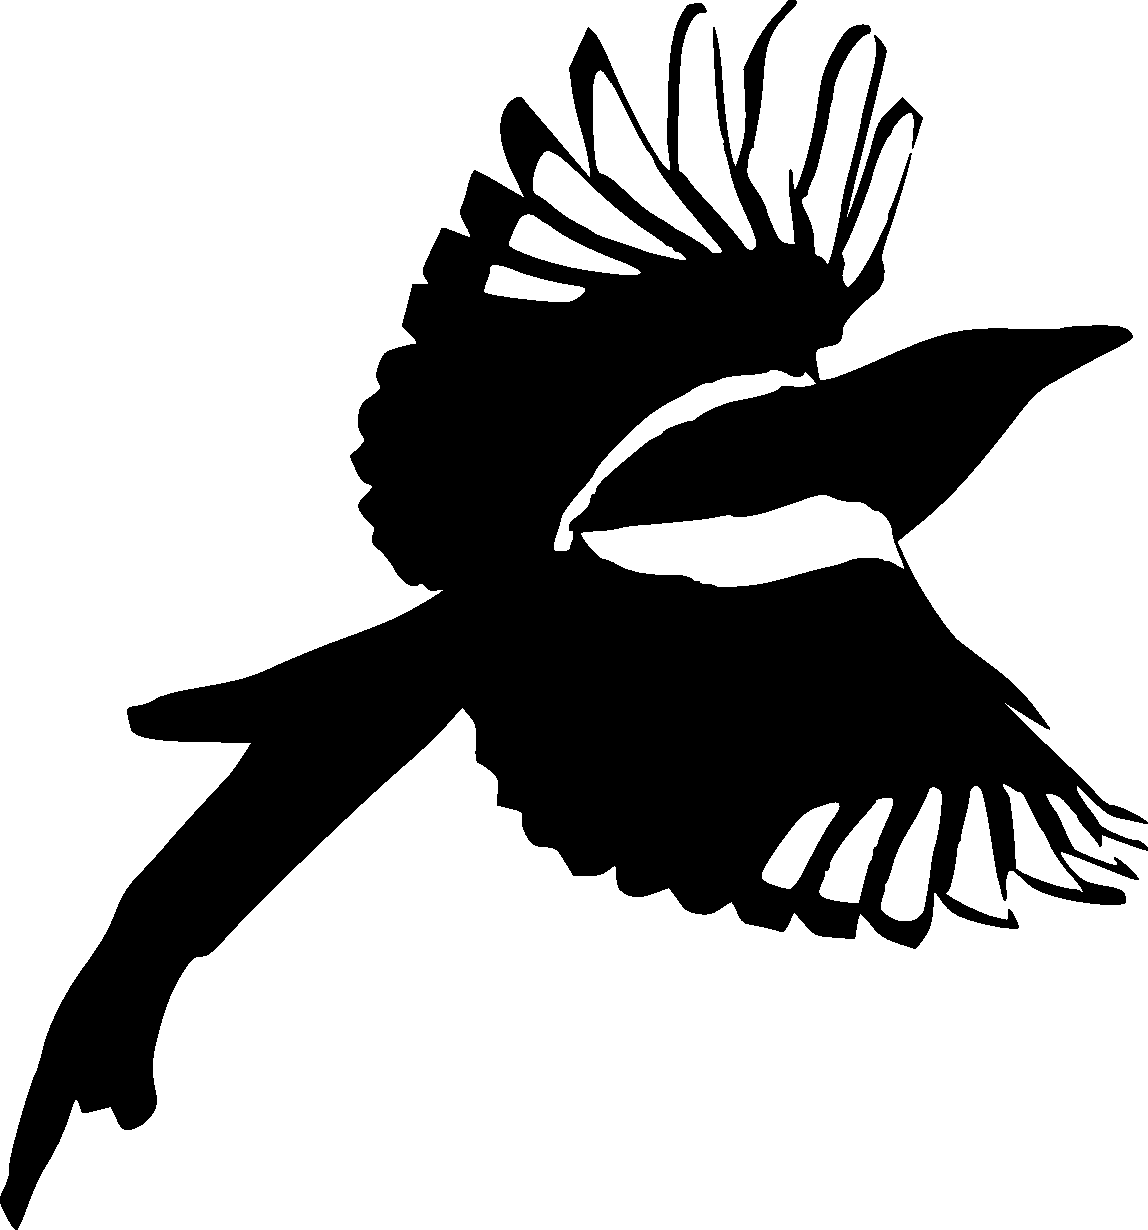
\includegraphics[height=0.7em]{img/magpie.pdf}}gpie} 
% }